% =====================================================================
%  Guía de laboratorio — IEL04 — Circuitos Eléctricos I, semana 8
%  Escrita por src/guia_laboratorio.py con la plantilla institucional
%  (config/framework_iub/guia-laboratorio/: guialabiub.sty e img/, copiados a esta carpeta).
%
%  Compilar con:  pdflatex -> biber -> pdflatex -> pdflatex
%  (En Overleaf: compilador pdfLaTeX; biber se ejecuta solo.)
% =====================================================================
\documentclass[12pt]{article}

% Opciones: [sinmarca] quita la marca de agua; [borrador] muestra márgenes
%           [ieee] referencias IEEE (por defecto); [apa] referencias APA 7
\usepackage{guialabiub}

% ------- Tablas, diagramas de flujo, circuitos y gráficas (todo en LaTeX) -------
% (la plantilla no los trae; los estilos y la paleta son los del .tex del temario)
\usepackage{colortbl}                    % encabezado #121023 y filas alternas en las tablas
\usepackage{xltabular}                   % la tabla de materiales se parte entre páginas
\usepackage{tikz}
\usetikzlibrary{arrows.meta,positioning,shapes.geometric,shapes.misc}
\usepackage[siunitx,RPvoltages]{circuitikz}
\usepackage{pgfplots}
\pgfplotsset{compat=1.18}
\usepackage{adjustbox}

% Paleta del Manual de Identidad Visual IUB 2025 (los colores del manual y sus tintes)
\definecolor{iubnavy}{HTML}{121023}
\definecolor{iubyellow}{HTML}{FFDF2D}
\definecolor{iubwhite}{HTML}{FFFFFF}
\definecolor{iubblue}{HTML}{00ADE7}
\definecolor{iuborange}{HTML}{E39037}
\definecolor{iubgreen}{HTML}{3B9C6D}
\colorlet{iubgris}{iubnavy!18}
\colorlet{iubgrisoscuro}{iubnavy!60}
\colorlet{iubfondoazul}{iubblue!8}
\colorlet{iubfondonaranja}{iuborange!10}
\colorlet{iubfondoverde}{iubgreen!9}
\colorlet{iubfondogris}{iubnavy!5}
\colorlet{iubpurple}{iubnavy!45}
\pgfplotsset{cycle list={{iubblue, mark=*},{iuborange, mark=square*},{iubgreen, mark=triangle*},{iubnavy, mark=diamond*},{iubyellow, mark=pentagon*}}}

% Estilos de los diagramas de flujo (TikZ) y de las gráficas (pgfplots)
\tikzset{
  dcaja/.style={draw=iubblue, fill=iubfondoazul, line width=1pt, rounded corners=1pt, align=center, inner sep=2pt, text=iubnavy},
  destado/.style={draw=iubblue, fill=iubfondoazul, line width=1pt, rounded corners=6pt, align=center, inner sep=2pt, text=iubnavy},
  ddecision/.style={draw=iuborange, fill=iubfondonaranja, line width=1pt, diamond, aspect=1.6, align=center, inner sep=1pt, text=iubnavy},
  dterminal/.style={draw=iubgreen, fill=iubfondoverde, line width=1pt, rounded rectangle, align=center, inner sep=2pt, text=iubnavy},
  dflecha/.style={-{Stealth[length=2.4mm]}, line width=0.9pt, draw=iubnavy},
  drotulo/.style={font=\footnotesize, text=iubgrisoscuro, fill=white, fill opacity=0.92, text opacity=1, inner sep=1.5pt},
}
\pgfplotsset{iubejes/.style={width=0.9\linewidth, height=6.2cm, grid=major, grid style={iubgris}, axis lines*=left, axis line style={iubnavy}, tick label style={font=\small}, label style={font=\small}, title style={font=\bfseries\small}, legend cell align=left, legend style={draw=none, fill=none, font=\small, anchor=north, legend columns=-1, /tikz/every even column/.append style={column sep=8pt}}, unbounded coords=jump}}

% --------------------------- Bibliografía ----------------------------
\addbibresource{IEL04-semana08.bib}

% --------------------------- Datos de la guía -------------------------
\facultad{Facultad de Ingenierías}
\modulo{IEL04 --- Circuitos Eléctricos I}
\docente{Ing. Sergio Martinez Castilla}

\begin{document}

% Orden de la bibliografía: el mismo del .md (biblatex numera por orden de primera cita)
\nocite{ref1,ref2,ref3}

\datosguia
\lineablanco

% Título de la práctica y ficha de la sesión
{\centering\bfseries Guía de laboratorio: Circuitos RL en serie y en paralelo con la bobina real: tensiones, corrientes y ángulos a 10 kHz\par}
\lineablanco
\textbf{Semana:} 8 de 14 \quad \textbf{Resultado de aprendizaje:} IEL04-RA3 \quad \textbf{Práctica:} propuesta a partir de la bibliografía \cite{ref1}, \cite{ref2}, \cite{ref3} \quad \textbf{Duración:} \SI{240}{\minute}
\lineablanco
La práctica corresponde a la sesión teórica de la semana 8, \guillemotleft{}Circuitos RL en serie y en paralelo: reactancia inductiva, impedancia y leyes de Kirchhoff con la bobina real\guillemotright{}, y reproduce su caso de estudio: con la bobina L3 del kit y un resistor de 680 \ensuremath{\Omega} se miden, a 10 kHz y 5,00 V eficaces, las tensiones y el ángulo del circuito en serie y las corrientes y el ángulo del circuito en paralelo, y se comparan con el cálculo que incluye la resistencia de devanado y con el cálculo ideal. No hay un manual de laboratorio asignado al RA IEL04-RA3, por lo que la práctica se propone a partir de la bibliografía cargada: Floyd trata la reactancia inductiva y el análisis de circuitos RL en serie y en paralelo \cite{ref1}, Boylestad los circuitos de ca R-L \cite{ref2} y Deorsola el circuito RL y las leyes de Kirchhoff con fasores \cite{ref3}.

% ---------------------------------------------------------------------
\section{Objetivos}\label{sec:objetivos}
\textbf{Objetivo general:} Verificar experimentalmente las leyes de Kirchhoff en circuitos RL en serie y en paralelo con una bobina real.
\lineablanco
\textbf{Objetivos específicos:}
\begin{itemize}
  \item Identificar y verificar con instrumentos la bobina y el resistor del circuito, incluida la resistencia de devanado. \emph{(CE1)}
  \item Medir las tensiones en el resistor y en la bobina, y las corrientes de rama, con el multímetro de verdadero valor eficaz. \emph{(CE2)}
  \item Medir el ángulo de fase de los circuitos RL en serie y en paralelo, y compararlo con el cálculo con resistencia de devanado y con el cálculo ideal. \emph{(CE3)}
\end{itemize}

% ---------------------------------------------------------------------
\section{Materiales y Equipos}\label{sec:materiales}
% --- Tabla: materiales y equipos (9; xltabular repite el encabezado si se parte) ---
\arrayrulecolor{iubnavy}
\begin{xltabular}{\linewidth}{>{\raggedleft\arraybackslash}p{0.6cm} >{\raggedright\arraybackslash}X >{\raggedright\arraybackslash}X >{\raggedleft\arraybackslash}p{2.2cm}}
\caption{Materiales y equipos de la práctica}\label{tab:materiales} \\
\rowcolor{iubnavy} \textcolor{white}{\textbf{\#}} & \textcolor{white}{\textbf{Material o equipo}} & \textcolor{white}{\textbf{Especificación}} & \textcolor{white}{\textbf{Cantidad}} \\
\endfirsthead
\rowcolor{iubnavy} \textcolor{white}{\textbf{\#}} & \textcolor{white}{\textbf{Material o equipo}} & \textcolor{white}{\textbf{Especificación}} & \textcolor{white}{\textbf{Cantidad}} \\
\endhead
\bottomrule
\endlastfoot
  1 & Bobina L3 del kit & 103K, 10,4 mH y 24,6 \ensuremath{\Omega} medidos & 1 \\
  \rowcolor{iubfondogris} 2 & Resistor & 680 \ensuremath{\Omega} & 1 \\
  3 & Resistor sensor de corriente & 10 \ensuremath{\Omega} & 1 \\
  \rowcolor{iubfondogris} 4 & Generador de funciones & --- & 1 \\
  5 & Osciloscopio de dos canales con puntas \texttimes{}10 & --- & 1 \\
  \rowcolor{iubfondogris} 6 & Multímetro digital de verdadero valor eficaz & --- & 2 \\
  7 & Medidor LCR & --- & 1 \\
  \rowcolor{iubfondogris} 8 & Protoboard & --- & 1 \\
  9 & Cables de conexión & --- & 12 \\
\end{xltabular}

% ---------------------------------------------------------------------
\section{Procedimiento}\label{sec:procedimiento}
La práctica ocupa el bloque de 2 h de laboratorio de la sesión y se realiza en grupos de tres estudiantes, con tres roles que rotan entre etapas: quien monta y opera el circuito, quien mide y quien registra y verifica los cálculos. Antes de energizar cualquier montaje, el docente o el monitor revisa la conexión. Cada etapa abre con su diagrama de flujo, que muestra la secuencia y las comprobaciones de un vistazo, y sigue con sus pasos numerados; cada paso indica cuánto dura, qué debe observarse para saber que salió bien y qué hacer si no. Los valores numéricos de la sesión teórica sirven de referencia: las lecturas propias del grupo se registran en las tablas de la sección de análisis.
\lineablanco
% --- Etapa 1: Preparación y cálculo previo (2 pasos) ---
\subsection{Preparación y cálculo previo (\SI{18}{\minute})}\label{sec:etapa-1}
\begin{pasos}
  \item \textbf{Paso~1:} Verificar la bobina L3 con el medidor LCR (inductancia) y el ohmímetro (resistencia de devanado), y el resistor de 680 \ensuremath{\Omega} con el ohmímetro. \emph{(aprox.~\SI{6}{\minute})} \textbf{Comprobación:} L3 debe leer cerca de 10,4 mH y 24,6 \ensuremath{\Omega}, y el resistor cerca de 676 \ensuremath{\Omega}; si no, anotar los valores nuevos para los cálculos.
  \item \textbf{Paso~2:} Calcular a 10 kHz la reactancia $X_L = 2\pi f L$, la impedancia del circuito en serie con y sin la resistencia de devanado, y las corrientes del circuito en paralelo. \emph{(aprox.~\SI{12}{\minute})} \textbf{Comprobación:} Debe obtenerse $X_L$ cerca de 653 \ensuremath{\Omega} y una corriente en serie cerca de 5,2 mA.
% ecuación del paso 2: Reactancia inductiva e impedancia del RL en serie con la bobina real:
\par Reactancia inductiva e impedancia del RL en serie con la bobina real:
\begin{equation}
  X_L = 2\pi f L, \qquad Z = \sqrt{(R + R_W)^2 + X_L^2}
  \label{eq:paso-2}
\end{equation}
donde $X_L$ y $Z$ en ohmios (\ensuremath{\Omega}), $f$ en Hz, $L$ en H, $R$ y $R_W$ en \ensuremath{\Omega}.
\end{pasos}
% --- Etapa 2: Circuito RL en serie (4 pasos) ---
\subsection{Circuito RL en serie (\SI{27}{\minute})}\label{sec:etapa-2}
% --- Figura 1: diagrama de flujo de la etapa 2 (TikZ, con la paleta IUB) ---
\begin{figure}[H]
  \centering
\begin{adjustbox}{max width=\linewidth}
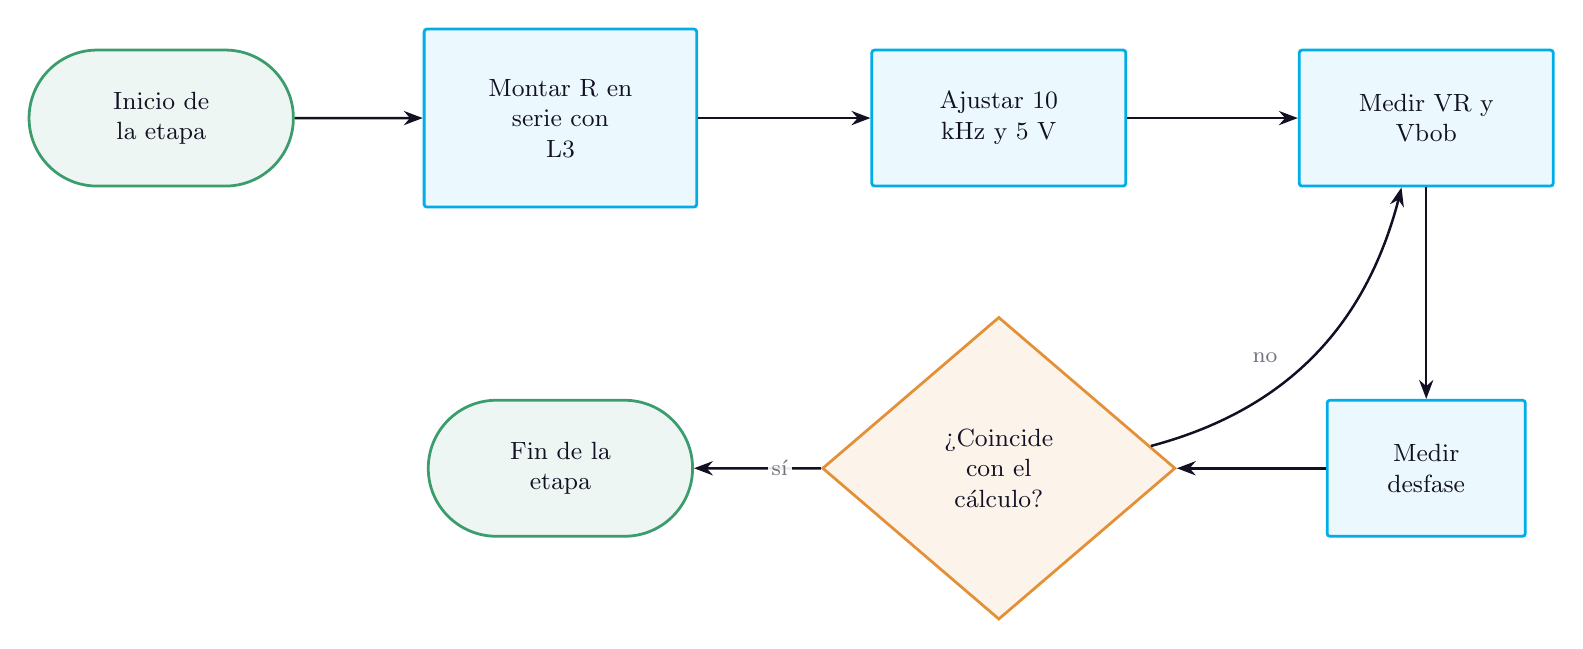
\begin{tikzpicture}[x=1in, y=1in, font=\small]
  % nodos (centro en pulgadas, con el tamano que calcula figuras.py)
  \node[dterminal, minimum width=1.377in, minimum height=0.680in] (n0) at (0.689,-0.445) {Inicio de \\ la etapa};  % ini
  \node[dcaja, minimum width=1.363in, minimum height=0.890in] (n1) at (2.685,-0.445) {Montar R en \\ serie con \\ L3};  % a0
  \node[dcaja, minimum width=1.270in, minimum height=0.680in] (n2) at (4.877,-0.445) {Ajustar 10 \\ kHz y 5 V};  % a1
  \node[dcaja, minimum width=1.270in, minimum height=0.680in] (n3) at (7.014,-0.445) {Medir VR y \\ Vbob};  % a2
  \node[dcaja, minimum width=0.991in, minimum height=0.680in] (n4) at (7.014,-2.196) {Medir \\ desfase};  % a3
  \node[ddecision, minimum width=1.766in, minimum height=1.513in] (n5) at (4.877,-2.196) {\textquestiondown{}Coincide \\ con el \\ cálculo?};  % dec
  \node[dterminal, minimum width=1.377in, minimum height=0.680in] (n6) at (2.685,-2.196) {Fin de la \\ etapa};  % fin
  % flechas (las de retorno, curvas)
  \draw[dflecha] (n0) -- (n1);
  \draw[dflecha] (n1) -- (n2);
  \draw[dflecha] (n2) -- (n3);
  \draw[dflecha] (n3) -- (n4);
  \draw[dflecha] (n4) -- (n5);
  \draw[dflecha] (n5) -- (n6);
  \draw[dflecha] (n5) to[bend right=31] (n3);
  % rotulos de las flechas (donde no caen sobre un nodo)
  \node[drotulo] at (3.781,-2.196) {sí};
  \node[drotulo] at (6.208,-1.641) {no};
\end{tikzpicture}
\end{adjustbox}
  \caption{Diagrama de flujo de la etapa 2: Circuito RL en serie}
  \label{fig:flujo-2}
\end{figure}
\begin{pasos}
  \item \textbf{Paso~3:} Montar el resistor en serie con L3, con la bobina del lado de tierra. \emph{(aprox.~\SI{5}{\minute})} \textbf{Comprobación:} El docente revisa el montaje antes de energizar. \textbf{Seguridad:} Montar con el generador apagado.
% figura del paso 3: Circuito RL en serie con la bobina real (inductancia y resistencia de devanado) (circuito en circuitikz)
\par\medskip\noindent
\begin{minipage}{\linewidth}
  \centering
  \begin{adjustbox}{max width=\linewidth}
    \begin{circuitikz}[color=iubnavy]
    \draw (0,0) to[sV, l=$v_s$] (0,3) to[R, l_=$R$, v^=$v_R$] (4,3) to[L, l=$L_3$] (4,1.5) to[R, l=$R_W$] (4,0) -- (0,0); \draw (0,0) node[ground]{};
    \end{circuitikz}
  \end{adjustbox}
  \captionof{figure}{Circuito RL en serie con la bobina real (inductancia y resistencia de devanado)}\label{fig:paso-3}
\end{minipage}
\par\medskip
  \item \textbf{Paso~4:} Ajustar el generador a una onda sinusoidal de 10 kHz y medir con el osciloscopio y con el multímetro de verdadero valor eficaz que la tensión en los bornes del circuito, con el circuito conectado, sea de 5,00 V eficaces. \emph{(aprox.~\SI{6}{\minute})} \textbf{Comprobación:} El multímetro debe indicar 5,00 V y el osciloscopio una sinusoide sin distorsión; si la tensión baja al conectar el circuito, reajustar la amplitud con el circuito conectado.
  \item \textbf{Paso~5:} Medir con el multímetro de verdadero valor eficaz la tensión en el resistor y la tensión entre los terminales de la bobina. \emph{(aprox.~\SI{8}{\minute})} \textbf{Comprobación:} Las lecturas deben estar cerca de 3,53 V y 3,41 V; su suma aritmética supera 5 V.
  \item \textbf{Paso~6:} Medir con el osciloscopio el desfase entre la tensión de la fuente y la del resistor y calcular el ángulo. \emph{(aprox.~\SI{8}{\minute})} \textbf{Comprobación:} La corriente debe atrasar a la tensión unos 43\textdegree{}; si el ángulo se acerca a 44\textdegree{}, comprobar si se omitió la resistencia de devanado en el cálculo.
\end{pasos}
% --- Etapa 3: Circuito RL en paralelo (3 pasos) ---
\subsection{Circuito RL en paralelo (\SI{28}{\minute})}\label{sec:etapa-3}
% --- Figura 3: diagrama de flujo de la etapa 3 (TikZ, con la paleta IUB) ---
\begin{figure}[H]
  \centering
\begin{adjustbox}{max width=\linewidth}
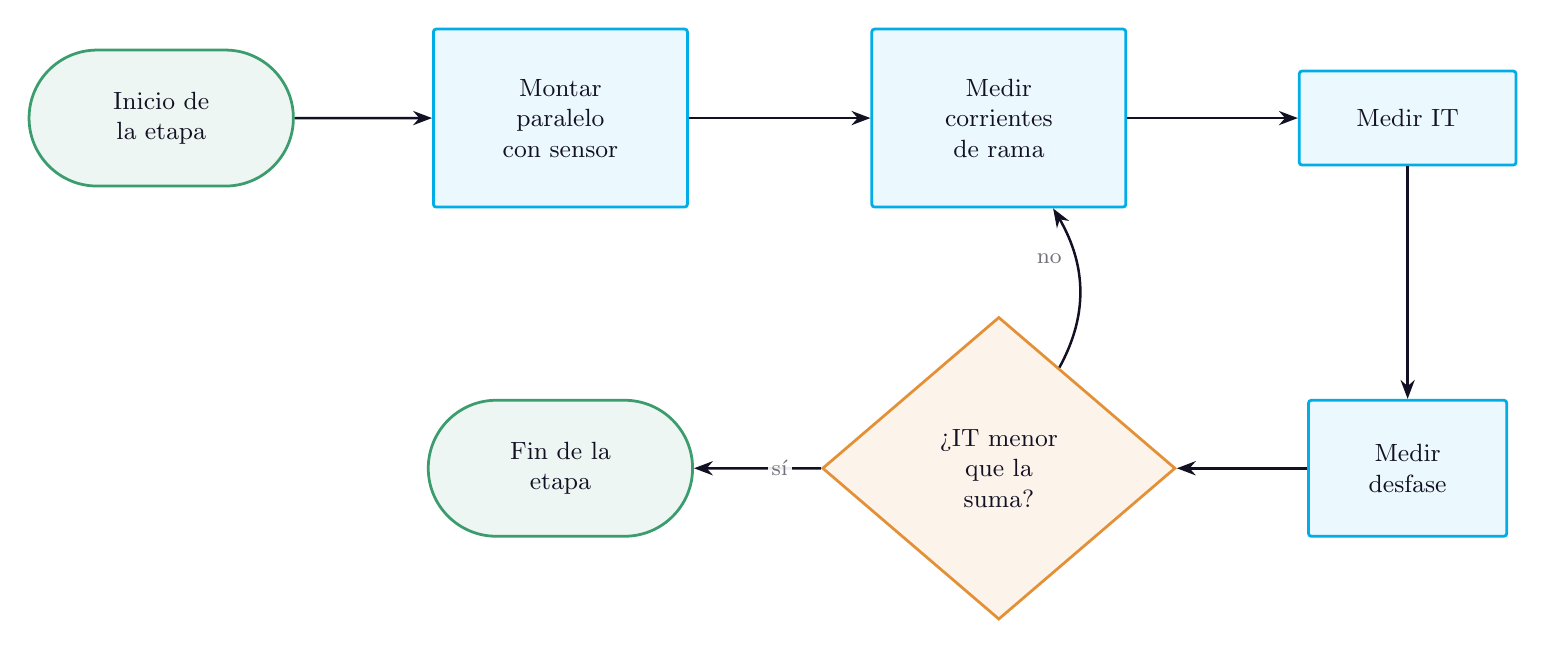
\begin{tikzpicture}[x=1in, y=1in, font=\small]
  % nodos (centro en pulgadas, con el tamano que calcula figuras.py)
  \node[dterminal, minimum width=1.377in, minimum height=0.680in] (n0) at (0.689,-0.445) {Inicio de \\ la etapa};  % ini
  \node[dcaja, minimum width=1.270in, minimum height=0.890in] (n1) at (2.685,-0.445) {Montar \\ paralelo \\ con sensor};  % a0
  \node[dcaja, minimum width=1.270in, minimum height=0.890in] (n2) at (4.877,-0.445) {Medir \\ corrientes \\ de rama};  % a1
  \node[dcaja, minimum width=1.084in, minimum height=0.470in] (n3) at (6.921,-0.445) {Medir IT};  % a2
  \node[dcaja, minimum width=0.991in, minimum height=0.680in] (n4) at (6.921,-2.196) {Medir \\ desfase};  % a3
  \node[ddecision, minimum width=1.766in, minimum height=1.513in] (n5) at (4.877,-2.196) {\textquestiondown{}IT menor \\ que la \\ suma?};  % dec
  \node[dterminal, minimum width=1.377in, minimum height=0.680in] (n6) at (2.685,-2.196) {Fin de la \\ etapa};  % fin
  % flechas (las de retorno, curvas)
  \draw[dflecha] (n0) -- (n1);
  \draw[dflecha] (n1) -- (n2);
  \draw[dflecha] (n2) -- (n3);
  \draw[dflecha] (n3) -- (n4);
  \draw[dflecha] (n4) -- (n5);
  \draw[dflecha] (n5) -- (n6);
  \draw[dflecha] (n5) to[bend right=31] (n2);
  % rotulos de las flechas (donde no caen sobre un nodo)
  \node[drotulo] at (3.781,-2.196) {sí};
  \node[drotulo] at (5.129,-1.146) {no};
\end{tikzpicture}
\end{adjustbox}
  \caption{Diagrama de flujo de la etapa 3: Circuito RL en paralelo}
  \label{fig:flujo-3}
\end{figure}
\begin{pasos}
  \item \textbf{Paso~7:} Desenergizar y montar el resistor y L3 en paralelo, con el resistor sensor en serie con la fuente del lado de tierra. \emph{(aprox.~\SI{6}{\minute})} \textbf{Comprobación:} El docente revisa el montaje. \textbf{Seguridad:} Desenergizar antes de modificar el montaje.
% figura del paso 7: Circuito RL en paralelo con el amperímetro en serie con la fuente (circuito en circuitikz)
\par\medskip\noindent
\begin{minipage}{\linewidth}
  \centering
  \begin{adjustbox}{max width=\linewidth}
    \begin{circuitikz}[color=iubnavy]
    \draw (0,0) to[sV, l=$v_s$] (0,3) to[ammeter, l=$I_T$] (3,3) to[R, l=$R$] (3,0) -- (0,0); \draw (3,3) -- (6,3) to[L, l=$L_3$] (6,0) -- (3,0); \draw (0,0) node[ground]{};
    \end{circuitikz}
  \end{adjustbox}
  \captionof{figure}{Circuito RL en paralelo con el amperímetro en serie con la fuente}\label{fig:paso-7}
\end{minipage}
\par\medskip
  \item \textbf{Paso~8:} Con el circuito desenergizado, insertar el amperímetro en cada rama y en serie con la fuente, energizando para cada lectura, y anotar $I_R$, $I_{\mathrm{bob}}$ e $I_T$. \emph{(aprox.~\SI{15}{\minute})} \textbf{Comprobación:} Las lecturas deben estar cerca de 7,40 mA, 7,65 mA y 10,8 mA; $I_T$ debe ser menor que la suma aritmética.
  \item \textbf{Paso~9:} Medir con el osciloscopio el desfase entre la tensión de la fuente y la del resistor sensor. \emph{(aprox.~\SI{7}{\minute})} \textbf{Comprobación:} La corriente total debe atrasar a la tensión unos 45\textdegree{}.
\end{pasos}
% --- Etapa 4: Desmontaje y cierre (3 pasos) ---
\subsection{Desmontaje y cierre (\SI{10}{\minute})}\label{sec:etapa-4}
% --- Figura 5: diagrama de flujo de la etapa 4 (TikZ, con la paleta IUB) ---
\begin{figure}[H]
  \centering
\begin{adjustbox}{max width=\linewidth}
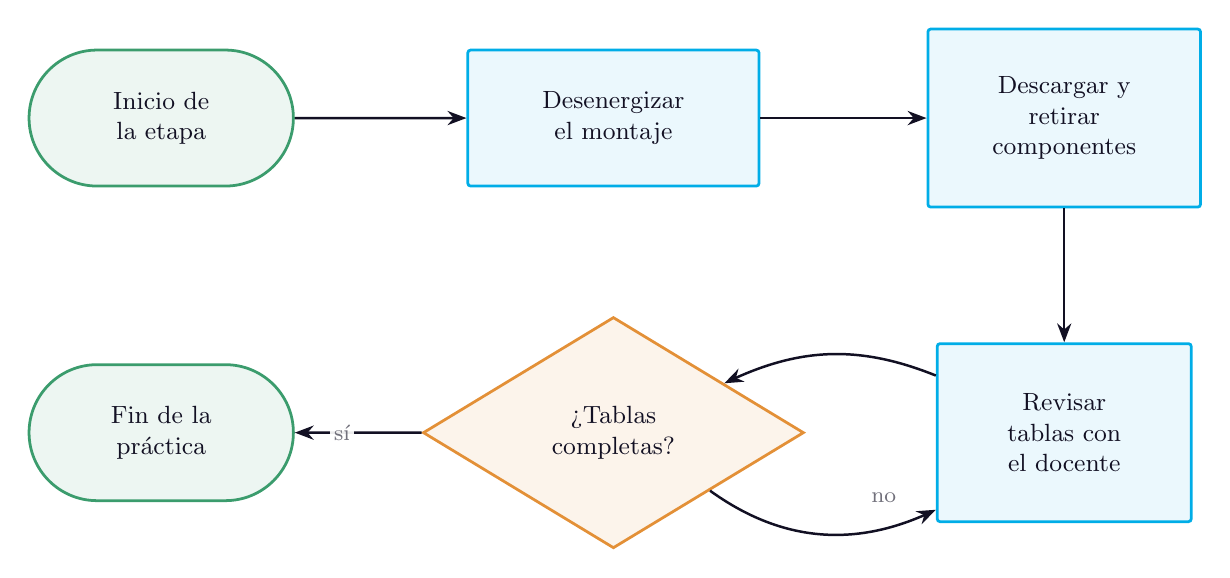
\begin{tikzpicture}[x=1in, y=1in, font=\small]
  % nodos (centro en pulgadas, con el tamano que calcula figuras.py)
  \node[dterminal, minimum width=1.377in, minimum height=0.680in] (n0) at (0.689,-0.445) {Inicio de \\ la etapa};  % ini
  \node[dcaja, minimum width=1.456in, minimum height=0.680in] (n1) at (2.950,-0.445) {Desenergizar \\ el montaje};  % a0
  \node[dcaja, minimum width=1.363in, minimum height=0.890in] (n2) at (5.204,-0.445) {Descargar y \\ retirar \\ componentes};  % a1
  \node[dcaja, minimum width=1.270in, minimum height=0.890in] (n3) at (5.204,-2.018) {Revisar \\ tablas con \\ el docente};  % a2
  \node[ddecision, minimum width=1.905in, minimum height=1.156in] (n4) at (2.950,-2.018) {\textquestiondown{}Tablas \\ completas?};  % dec
  \node[dterminal, minimum width=1.377in, minimum height=0.680in] (n5) at (0.689,-2.018) {Fin de la \\ práctica};  % fin
  % flechas (las de retorno, curvas)
  \draw[dflecha] (n0) -- (n1);
  \draw[dflecha] (n1) -- (n2);
  \draw[dflecha] (n2) -- (n3);
  \draw[dflecha] (n3) to[bend right=24] (n4);
  \draw[dflecha] (n4) -- (n5);
  \draw[dflecha] (n4) to[bend right=31] (n3);
  % rotulos de las flechas (donde no caen sobre un nodo)
  \node[drotulo] at (1.593,-2.018) {sí};
  \node[drotulo] at (4.302,-2.343) {no};
\end{tikzpicture}
\end{adjustbox}
  \caption{Diagrama de flujo de la etapa 4: Desmontaje y cierre}
  \label{fig:flujo-4}
\end{figure}
\begin{pasos}
  \item \textbf{Paso~10:} Apagar el generador de funciones y la fuente, desconectar las puntas del osciloscopio y retirar la alimentación del protoboard. \emph{(aprox.~\SI{3}{\minute})} \textbf{Comprobación:} Ningún indicador de salida debe quedar encendido en el generador ni en la fuente. \textbf{Seguridad:} Desenergizar siempre antes de retirar componentes.
  \item \textbf{Paso~11:} Descargar los condensadores del montaje con la resistencia de descarga, retirar los componentes y devolverlos al kit del grupo con su rótulo. \emph{(aprox.~\SI{4}{\minute})} \textbf{Comprobación:} El kit debe quedar completo, con cada componente en su lugar y con su valor medido anotado.
  \item \textbf{Paso~12:} Revisar con el docente las tablas de registro antes de abandonar el banco. \emph{(aprox.~\SI{3}{\minute})} \textbf{Comprobación:} Las tablas deben estar completas y con unidades; si falta un dato, repetir esa medición antes de desmontar el instrumento.
\end{pasos}

% ---------------------------------------------------------------------
\section{Cuestiones a Resolver}\label{sec:cuestiones}
\begin{enumerate}
  \item \textquestiondown{}En qué circuito, serie o paralelo, pesa más la resistencia de devanado de la bobina, y por qué?
  \item \textquestiondown{}Cuánto se apartan las mediciones del cálculo ideal y cuánto del cálculo con resistencia de devanado?
  \item \textquestiondown{}Por qué la tensión medida en la bobina no está adelantada exactamente 90\textdegree{} respecto de la corriente?
  \item \textquestiondown{}Cómo cambiaría el efecto de la resistencia de devanado si la práctica se hiciera a 1 kHz en lugar de 10 kHz?
\end{enumerate}

% ---------------------------------------------------------------------
\section{Análisis de Resultados}\label{sec:analisis}
Presentar en la tabla de registro, para cada magnitud de los dos circuitos, el cálculo con resistencia de devanado, el cálculo ideal, la medición y la diferencia porcentual con el primero.
\lineablanco
Dibujar el diagrama fasorial de tensiones del circuito en serie, con la tensión de la bobina real formada por su caída resistiva y su caída reactiva, y el de corrientes del circuito en paralelo; comprobar ambas sumas con las lecturas.
% --- Tabla de registro 1: Circuito RL en serie a 10 kHz (4 filas vacías para registrar en el banco) ---
\begin{table}[H]
  \centering
  \caption{Circuito RL en serie a 10 kHz}
  \label{tab:registro-1}
  \arrayrulecolor{iubnavy}
  \begin{tabularx}{\linewidth}{>{\raggedright\arraybackslash}X>{\raggedright\arraybackslash}X>{\raggedright\arraybackslash}X>{\raggedright\arraybackslash}X>{\raggedright\arraybackslash}X>{\raggedright\arraybackslash}X}
    \rowcolor{iubnavy} \textcolor{white}{\textbf{Magnitud}} & \textcolor{white}{\textbf{Cálculo con RW}} & \textcolor{white}{\textbf{Cálculo ideal}} & \textcolor{white}{\textbf{Medido}} & \textcolor{white}{\textbf{Unidad}} & \textcolor{white}{\textbf{Diferencia (\%)}} \\
    \rule{0pt}{0.8cm} & & & & & \\
    \rowcolor{iubfondogris} \rule{0pt}{0.8cm} & & & & & \\
    \rule{0pt}{0.8cm} & & & & & \\
    \rowcolor{iubfondogris} \rule{0pt}{0.8cm} & & & & & \\
    \bottomrule
  \end{tabularx}
\end{table}
% --- Tabla de registro 2: Circuito RL en paralelo a 10 kHz (4 filas vacías para registrar en el banco) ---
\begin{table}[H]
  \centering
  \caption{Circuito RL en paralelo a 10 kHz}
  \label{tab:registro-2}
  \arrayrulecolor{iubnavy}
  \begin{tabularx}{\linewidth}{>{\raggedright\arraybackslash}X>{\raggedright\arraybackslash}X>{\raggedright\arraybackslash}X>{\raggedright\arraybackslash}X>{\raggedright\arraybackslash}X>{\raggedright\arraybackslash}X}
    \rowcolor{iubnavy} \textcolor{white}{\textbf{Magnitud}} & \textcolor{white}{\textbf{Cálculo con RW}} & \textcolor{white}{\textbf{Cálculo ideal}} & \textcolor{white}{\textbf{Medido}} & \textcolor{white}{\textbf{Unidad}} & \textcolor{white}{\textbf{Diferencia (\%)}} \\
    \rule{0pt}{0.8cm} & & & & & \\
    \rowcolor{iubfondogris} \rule{0pt}{0.8cm} & & & & & \\
    \rule{0pt}{0.8cm} & & & & & \\
    \rowcolor{iubfondogris} \rule{0pt}{0.8cm} & & & & & \\
    \bottomrule
  \end{tabularx}
\end{table}

% ---------------------------------------------------------------------
\section{Conclusiones}\label{sec:conclusiones}
Concluir si las leyes de Kirchhoff se cumplen en forma fasorial en los dos circuitos y cuál de los dos modelos de la bobina (real o ideal) reproduce mejor las mediciones, explicando el papel de la resistencia de devanado; relacionar la práctica con los criterios de medición en circuitos resistivos, inductivos y RL del RA.
\lineablanco
\begin{itemize}
  \item \textquestiondown{}Qué modelo de la bobina explicó mejor los ángulos medidos?
  \item \textquestiondown{}Qué diferencia hubo entre el comportamiento en serie y en paralelo?
  \item \textquestiondown{}Qué precaución del montaje fue determinante?
\end{itemize}

% ---------------------------------------------------------------------
\section{Recomendaciones de Seguridad}\label{sec:seguridad}
\begin{itemize}
  \item Conectar las tierras de las dos puntas del osciloscopio a un mismo nodo de referencia: unirlas a nodos distintos cortocircuita el elemento que queda entre ellas.
  \item Insertar el amperímetro en serie con la rama solo con el circuito desenergizado y con el instrumento en la función y la escala de corriente; nunca conectarlo en paralelo con la fuente.
  \item Desenergizar antes de cambiar del montaje en serie al montaje en paralelo.
  \item No interrumpir bruscamente la corriente de la bobina con el circuito energizado.
\end{itemize}

% ---------------------------------------------------------------------
\section{Bibliografía}\label{sec:bibliografia}
% Las fuentes cargadas se citan en el texto con \cite{refN}; el \nocite del principio fija su orden y \nocite{*} incluye las demás del .bib.
\nocite{*}
\bibliografia

\end{document}
